\documentclass{exam}

\usepackage[margin=1in]{geometry}

\usepackage{comment}
\usepackage{graphicx}
\usepackage{listings}
\usepackage{amsmath}
\usepackage{tikz}
\usetikzlibrary{matrix}

\newcommand{\addend}{\text{\textsl{\color{gray}{Addend}}}}
\newcommand{\augend}{\text{\textsl{\color{gray}{Augend}}}}
\newcommand{\sumOut}{\text{\textsl{\color{gray}{Sum}}}}



\pagestyle{headandfoot}
\firstpageheader{CSCI 389}{}{Binary and C Intro Assignment}
\runningheader{CSCI 389}{}{Binary and C Intro Assignment}


\begin{document}
\title{Binary and C Intro Assignment (Learning)}
\author{CSCI 389: Computer Systems}
\date{Spring 2022}
\maketitle


This assignment is an opportunity to test your understanding of binary and C and receive feedback. 
Point values are assigned so that you can differentiate between large and small mistakes, but this assignment does not affect your grade. 

\textbf{Due Date:}
Wednesday, February 2nd at 10:00 am. 

\begin{questions}

\question[12]
\textbf{Converting Bases.}
Convert the following numbers to the specified base. 
\begin{parts}
\part[2]
Convert $209_{10}$ to binary. 
\part[2]
Convert $192_{10}$ to hexadecimal. 
\part[2]
Convert $10110001_{2}$ to decimal. 
\part[2]
Convert $1001101_{2}$ to hexadecimal. 
\part[2]
Convert $D3A7_{16}$ to decimal. 
\part[2]
Convert $83EF_{16}$ to binary. 
\end{parts}

\textbf{A.} The smallest base 2 number that fits in is $128$ which is $2^{7}$. $209-128=81$, the next fitting power of two is $64$ which is $2^6$. $81-64=17$, the next power of 2 is 16 which is $2^4$. The last power of two is 1 which is $2^0$,

The resulting number is: $1101 0001$

\textbf{B.} The first digit is $\lfloor192/16 \rfloor= 	12=C$  and the second digit is $192\%16=0$. Therefore the hex digit is $C0$

\textbf{C.} $2^0+ 2^4+2^5+2^7= 209$

\textbf{D.} Digits can be grouped together in groups of 4. The last four buts $1101$ is 13 and the remaining three $100$ represent 4. So in hex the number is $4D$ 

\textbf{E.} $7(16^0)+ 10(16^1)+3(16^2)+13(16^3)=54183$

\textbf{F.} $15(16^0)+ 14(16^1)+3(16^2)+8(16^3)=33775$

\question[4]
\textbf{Binary Addition.}
Show how to add $10001111_{2}$ and $01100101_{2}$ using binary arithmetic. 

This is a series of half adds, and if there happens to be three then in addition to the carry the digit is also set to true.


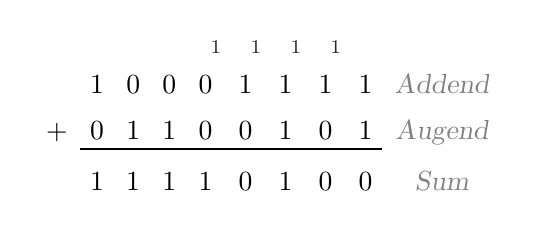
\begin{tikzpicture}[
    row 1/.style={font=\textsl,font=\scriptsize,black!85, anchor=west,
        inner sep=1.5pt},
    every node/.style={column sep=.5mm,row sep=1mm}]
    \matrix (m) [matrix of math nodes,
        nodes in empty cells,
        %nodes=draw
    ] 
    {
        &   &  &  & 1 & 1 & 1 & 1 &    &                   \\
        & 1 & 0 & 0 & 0 & 1 & 1 & 1 & 1 &[10mm]     \addend \\
    +  & 0 & 1 & 1 & 0 & 0 & 1 & 0 & 1 &           \augend \\ 
        & 1 & 1 & 1 & 1 & 0 & 1 & 0 & 0 &           \sumOut \\                                                  
    };

    \draw[-,color=black,semithick] (m-3-2.south west) -- (m-3-9.south east);

\end{tikzpicture}

Credits to %\href{https://tex.stackexchange.com/a/96764}{this} tex.stackechange post for the tikz code.

$1111 0100$

\question[4]
\textbf{Binary Multiplication.}
Show how to multiply $100110$ and $11001$ using binary arithmetic. 




\question[4]
\textbf{Latency and Bandwidth.}
Create the truth table for the following circuit:
\begin{center}
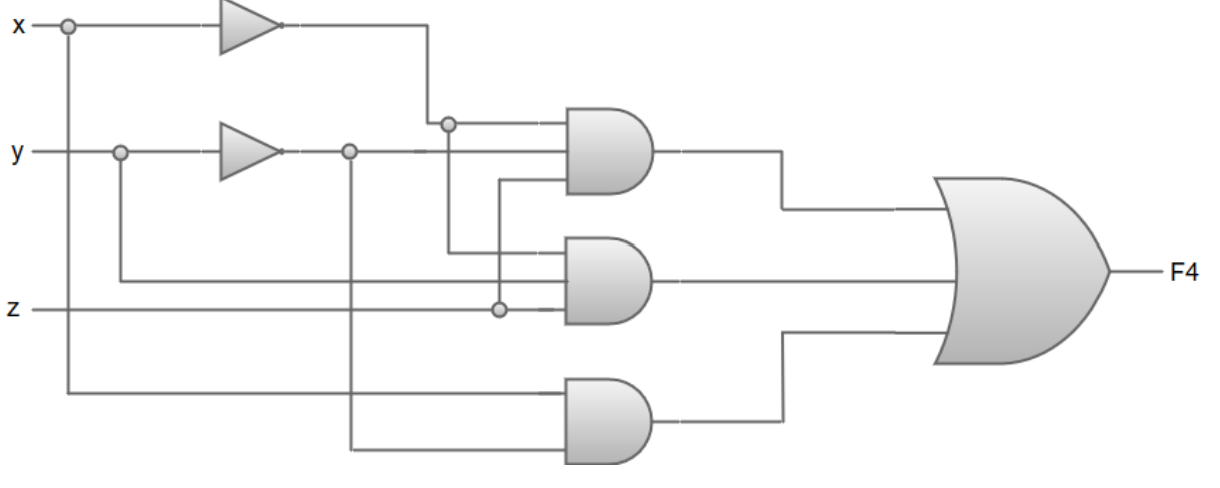
\includegraphics[width=0.6\textwidth{}]{circut.png}
\end{center}

$\begin{array}{|c c c | c|}
x&y&z&output\\
1&1&1&0\\
1&1&0&0\\
1&0&1&1\\ % by bottom
1&0&0&1\\ % by bottom
0&1&1&1\\ % by middle
0&1&0&0\\
0&0&1&1\\ % by top
0&0&0&0
\end{array}$


\question[16]
\textbf{C.}
Write C code that generates a list of random integers and computes the mean (as a real number). 
Your program should take as input two parameters, the length of the list, and a seed to generate the random numbers.
It should print out the list of integers and the calculated mean. 
Submit your code, as well as the makefile you used to compile it. 
\end{questions}




\end{document}